\chapter{Solution}
\label{ch:solution}
%Approx. 10 pages


\section{Implementation}

\subsection{Graph}
\begin{wrapfigure}{r}{5cm} % "placement and width parameter for the width of the image space.
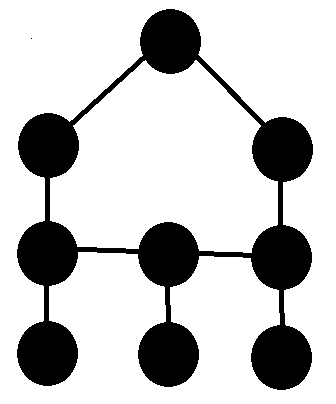
\includegraphics[width=40mm]{images/manuallyGraph.png}
\caption{\textit{The manually created graph}}
\label{smallgraph}
\end{wrapfigure}
The ship was modelled out as a graph with nodes and connections. There was used two different types of graph when testing, one which was created manually, shown in figure \ref{smallgraph}, and one that was randomly made each time. The nodes themselves represented a room on board the ship and the vertices from one node to another node represented the doors between the rooms. Every mode have some set of parameters set, how lethal it is or if it is an exit so the humans may get to safety. In this project we only used 1 or 0, where 1 was 100\% chance of death and 0 was 0\%, however we had implemented it so it was possible to set other chances. The reason for only choosing to have 0 or 1 during the testing, was to keep it simple, otherwise we might get overwhelmed in to many parameters that might impact the results. 


\subsection{Brute force}
The main algorithms that was used to find its way through the graph was a brute force, random and Ant Colony optimization. Brute force was the first algorithm to run, it went trough all the nodes going one step at the time and finding all the possible solutions for that node. When it was done it picked the shortest solution with the least likely hood of dying and set that as that nodes best route, then to the next node doing the same. Also if we used randomly generated graph, it checked if a human was in a node that had a possible way to an exit, if not it was updated so the human would not walk forever in random. 

\subsection{Random}
Random was simple in it's way that each human took one step and checked if they had reached an exit or died in that node. If the human started in a node that could not reach an exit node, it was counted as a dead human as it could not get to safety. In real situations, the possibility of people getting stuck like this is unlikely, however it might happen if parts of the ship collapses.

\subsection{Ant Colony Optimization}
In our Ant Colony algorithm, it started out the same way as random, by walking through the graph to find an exit. Once if do find an exit, it reports back in each node it visited and adds pheromones based on how long the path was and how lethal it was. In conventional ACO algoritems, it is only the path lenght that effects the pheromone update, however in our algoritmen the lethal nodes does too. If the ant path takes it trough a lethal node, the pheromones are reduced by how lethal the combined lethal nodes, since our nodes only had 1 or 0, it was reduced to 0 or not at all. When it have updated it pheromones the next and starts it journey, and walks around a bit less randomly, as the pheromones in the nodes gives a higher chance of choosing the same path as the previous ant. After some turns a path will develop as the AntSystem walks through the graph from an node to the exit, and when enough ants have walked trough the graph the best path will have the most pheromones and guide the ants on that path.

%\section{Proposed solution / algorithm}

%\subsection{The basic algorithm}

%\subsection{Discussion of design issues}


%\subsection{Algorithmic Enhancements}


%\subsection{Discussion of the Parameter Space}


%\section{Prototype}

%\section{Justification of Claim to Originality}

%\section{Valuation of Contribution}

%\section{Alternatives}
